We now look at two settings where our bias is likely to be present.  In the first one, we assume the
input graph is randomly perturbed version of a consistent clustering. In the second one, we do not
assume anything about such a consistent clustering but expect instead that the optimal solution is
\enquote{clear} enough that it does not change when weights are multiplicatively perturbed.

\paragraph{\pcc{} under noise}

As we have seen, assuming the Unique Games Conjecture, the \mmc{} problem, and therefore
the \pcc{} problem on a general graph, cannot be approximated to within a constant factor in the worst
case.  But maybe we can do better in the average case, which motivates the study of semi-random
model, where real graphs are seen as being obtained from the controlled perturbation of a perfectly
clusterable graph. In the simplest case, each edge sign is independently flipped with probability
$p \in [0, \shalf)$. This situation on complete graphs was considered in \autocite[Section
6]{Bansal2002}, showing a simple algorithm that with high probability makes
$\tilde{O}(n^\frac{3}{2})$ mistakes, and in \autocite[Theorem 2.6]{Ben-Dor99}, with an algorithm
recovering with high probability the planted partition of an unweighted graph in $O(n^2(\log n)^c)$,
where $c$ depends on the size of the smallest cluster and the noise probability.

\Textcite{Joachims2005} analyze a more refined weighted model, where weights are generated by a
probability distribution whose mean on true positive edges is larger than $\mu^+>0$ and whose mean
on true negative edges is smaller than $\mu^-<0$. They give a finite-sample bound on the number of
nodes misclustered w.r.t the planted partition as a function on the probability distribution
parameters. Indeed, as pointed out by \textcite{plantedAilon09}, independent and uniform noise is
not a good model of real situations, where the input of \pcc{}, \ie{} the similarity between nodes,
is often the result of a preprocessing, which may present strong correlations. Therefore, instead of
measuring the quality of a solution against the input (\ie{} the similarity information), they
argue it is more sensible to measure it against the (unknown) true optimal clustering that gave rise
to the input, and show that \ccpivot{} allows this, thanks to a new analysis. \Textcite{Mathieu2010}
also consider an adversarial model, where all edges are flipped with probability $p$ but the
adversary then decides whether to reveal the true sign or the flipped sign. On complete unweighted
graphs, they find a solution of \mind{} at most $1 + O(n^{-\nicefrac{1}{6}})$ times the optimal
whenever $p \leq \shalf - n^{-\nicefrac{1}{3}}$ by rounding the usual SDP solution. If, in addition,
there is no adversary, $p\leq\nicefrac{1}{3}$ and each planted cluster has at least
$\Theta(\sqrt{n})$ nodes, then the planted partition can be recovered exactly.
\Textcite{Makarychev2014} study the same adversarial model but on general weighted graphs, giving a PTAS
for \mind{} when $p\leq \nicefrac{1}{4}$. Under additional assumptions on the density of edges, they
present another algorithm that finds the ground truth clustering with an arbitrarily small
classification error.
% \footnote{They also mention a potentially interesting related work~\autocite{unobservedCC14}.}
% http://www.jmlr.org/papers/v15/chen14a.html
% \textcite{Noisy2CCLocality16} study the recovery of an arbitrary planted 2-partition under noisy
% measurement in special kind of graphs where each node is connected with a local neighborhood and
% show computationally efficient algorithms that only query an information theoretically optimal
% number of pair. I think it was extended in \url{https://doi.org/10.1109/TIT.2016.2600566}

\paragraph{\pcc{} under stability assumption}

Whereas clustering objective functions are \NPh{} to optimize, we expect meaningful instances
in which we are interested to have additional structure which allows for guaranteed polynomial time
algorithms. We refer the reader to a critical overview~\autocite{clusteringFeasibility15} of some
such notions of structure proposed recently. Informally, a general idea is that the clustering should not
change (or at least very little) if the data are slightly perturbed. For instance, a weighted graph
is \emph{$\alpha$-stable} (with $\alpha>1$) for some partition objective if its optimal partition
remains the same whenever every weight $w_i$ is multiplied by a factor $c_i$ between $1$ and
$\alpha$.
Another notion is the $(c, \epsilon)$-approximation stability. Formally, a dataset $X$ is $(c,
\epsilon)$-stable if, for an objective function $\Phi$, any clustering whose cost is within a factor
$c$ of the optimal cost $OPT_{\Phi}$ is $\epsilon$-close to the optimal clustering (as measured by
the fraction of points in which the two clustering disagree). When the objective is \mind{} on
complete graphs, \textcite{StableCC09} show that for $(1+\alpha, \epsilon)$-instances, the
approximation algorithms we describe in \autoref{ssub:cc_harness_approx} find a solution that is
$(\nicefrac{49}{\alpha} + 1)\epsilon$ close to the optimal clustering.

It is also possible to study the stability of a \pcc{} instance over a general graph w.r.t edge
weights via its canonical \mind{} LP. \Textcite{StableLP09} present a method to determine to which
extent the weights of a \pcc{} instance can be perturbed before the optimal solution changes.

\iffalse
\Textcite{StableCC17} provide a robust algorithm for $2-\nicefrac{2}{k}$-stable instance of
$k$-\textsc{Minimum Multiway Cut}, which therefore is not really useful in our case because I confused
multiway cut and multicut. To be fair, it seems I'm not the only one, \href{http://pages.cs.wisc.edu/~shuchi/papers/multicut-hardness-full.pdf}{on the hardness of
   approximating multicut}
   \enquote{multicut is known to be APX-hard
      (\href{https://pdfs.semanticscholar.org/1cf6/4c2bdd4f1c384a55910606a64c8d831a96ba.pdf}%
   {Dahlhaus et al. 1994}).} by that 1994 paper define the multiway cut problem, see
   \autoref{fig:cc_multiwhat}. \Textcite[Theorem 24]{Bansal2004} show that we can go from
   \textsc{Minimum Multiway Cut} to \pcc{} but I doubt about the other direction, mostly because
   \textsc{Minimum Multiway Cut} can actually be approximated with factor smaller than $1.3$.
   see \url{http://www.nowozin.net/sebastian/papers/nowozin2009lpstability.pdf} about LP multicut
   stability.
\begin{figure}[htpb]
   \centering
   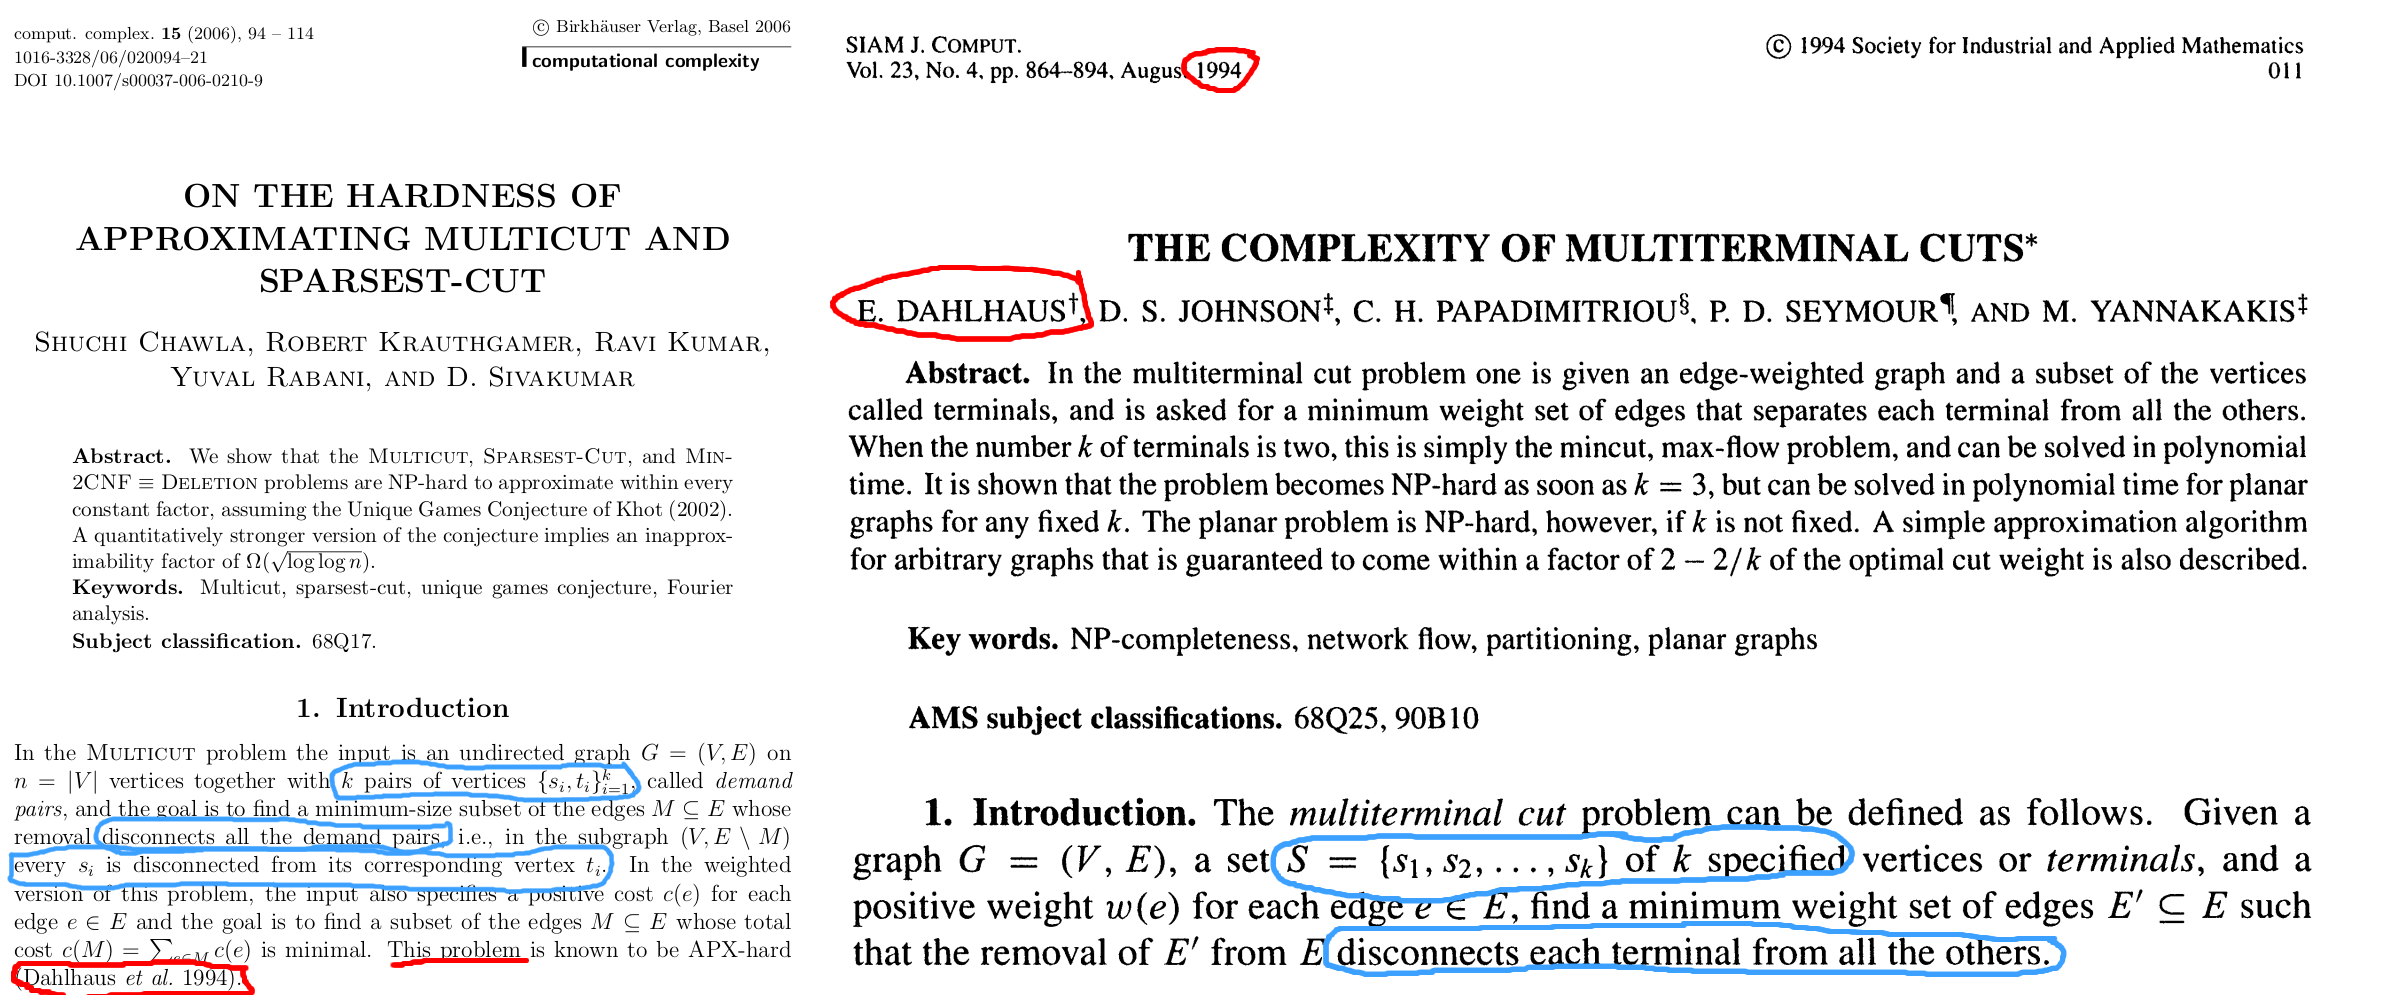
\includegraphics[width=0.9\linewidth]{assets/raw/multicut_vs_multiway.png}
   \caption{Confusing statement} \label{fig:cc_multiwhat}
\end{figure}
\fi


% \enquote{We prove that if the Unique Games Conjecture of Khot (2002) is true, then for every constant L > 0
% it is NP-hard to approximate Multicut within factor L. If a quantitatively stronger version of the
% conjecture is true, then Multicut is NP-hard to approximate within a factor of $\Omega(\sqrt{\log
% \log n})$.}

% It's probably limited because LP with a lot of constraints do not scale that well (someone claimed
% $O(n^{4.5})$)

% SDP Gaps and UGC Hardness for Multiway Cut, 0-Extension and Metric Labelling,
% On the Unique Games Conjecture: Subhash Khot
% under the UGC, one cannot get better than $O(\log n)$ approximation using LP or SDP relaxation.
